\chapter{Model}
Introduction to the chapter/worksheet.

\begin{flalign}
	\si{R_\phi} &=
	\begin{bmatrix}
		\ \si{1}                & \si{0}                & \si{0} \ \ \ \\ 
		\ \si{0}  				& \si{c(\phi)} 		& \si{s(\phi)}                 \ \ \ \\ 
		\ \si{0}                & \si{-s(\phi)}       & \si{s(\phi)}                  \ \ \  
	\end{bmatrix}  \nonumber \\
	\si{R_\theta} &=
	\begin{bmatrix}
		\ \si{c(\theta)}      & \si{0}       & \si{s(\theta)} \ \ \ \\ 
		\ \si{0}  				& \si{1} 	   & \si{0}                 \ \ \ \\ 
		\ \si{-s(\theta)}     & \si{0}       & \si{c(\theta)}                  \ \ \  
	\end{bmatrix}   \nonumber \\
	\si{R_\phi} &=
	\begin{bmatrix}
		\ \si{c(\psi)}                & \si{s(\psi)}                & \si{0} \ \ \ \\ 
		\ \si{-s(\psi)}  				& \si{c(\psi)} 		& \si{0}                 \ \ \ \\ 
		\ \si{0}                & \si{0}       & \si{1}                  \ \ \  
	\end{bmatrix} \nonumber \\
	\si{R_{\phi, \theta, \psi}} &=
	\begin{bmatrix}
		\ \si{c(\theta) \cdot c(\psi)}                & \si{c(\theta) \cdot s(\psi)}  & \si{-s(\theta)} \ \ \ \\ 
		\ \si{s(\phi) \cdot s(\theta) \cdot s(\psi) - c(\phi) \cdot s(\psi)}  	  & \si{s(\phi) \cdot s(\theta) \cdot s(\psi) + c(\phi) \cdot c(\psi)} 		& \si{s(\phi) \cdot c(\theta)}                 \ \ \ \\ 
		\ \si{c(\phi) \cdot s(\theta) \cdot c(\psi) + s(\phi) \cdot s(\psi)}  	  & \si{c(\phi) \cdot s(\theta) \cdot s(\psi) - s(\phi) \cdot c(\psi)} 		& \si{c(\phi) \cdot c(\theta)}                 \ \ \ 
	\end{bmatrix} 	
\end{flalign}

\begin{minipage}{\linewidth}
	\begin{minipage}{0.45\linewidth}
		\begin{figure}[H]
			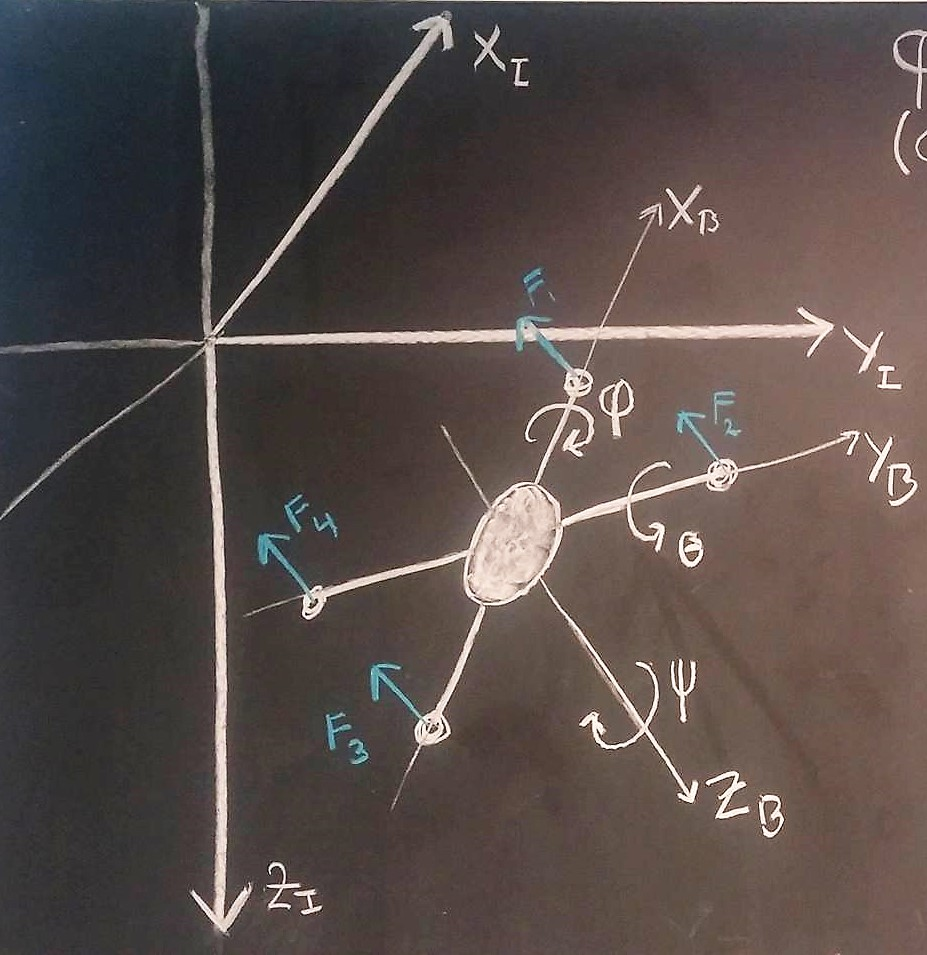
\includegraphics[scale=.27]{figures/drone_diagram}
			\centering
			\captionsetup{justification=centering}
			\captionof{figure}{Diagram of the quadcopter which includes inertial and body reference systems, as well as the references for the angles (roll, pitch and yaw) and the thrust forces produced by the propeller.}
			\label{PotentiometerResolution}
		\end{figure}
	\end{minipage}
	\hspace{0.03\linewidth}
	\begin{minipage}{0.45\linewidth}
		\begin{figure}[H]
			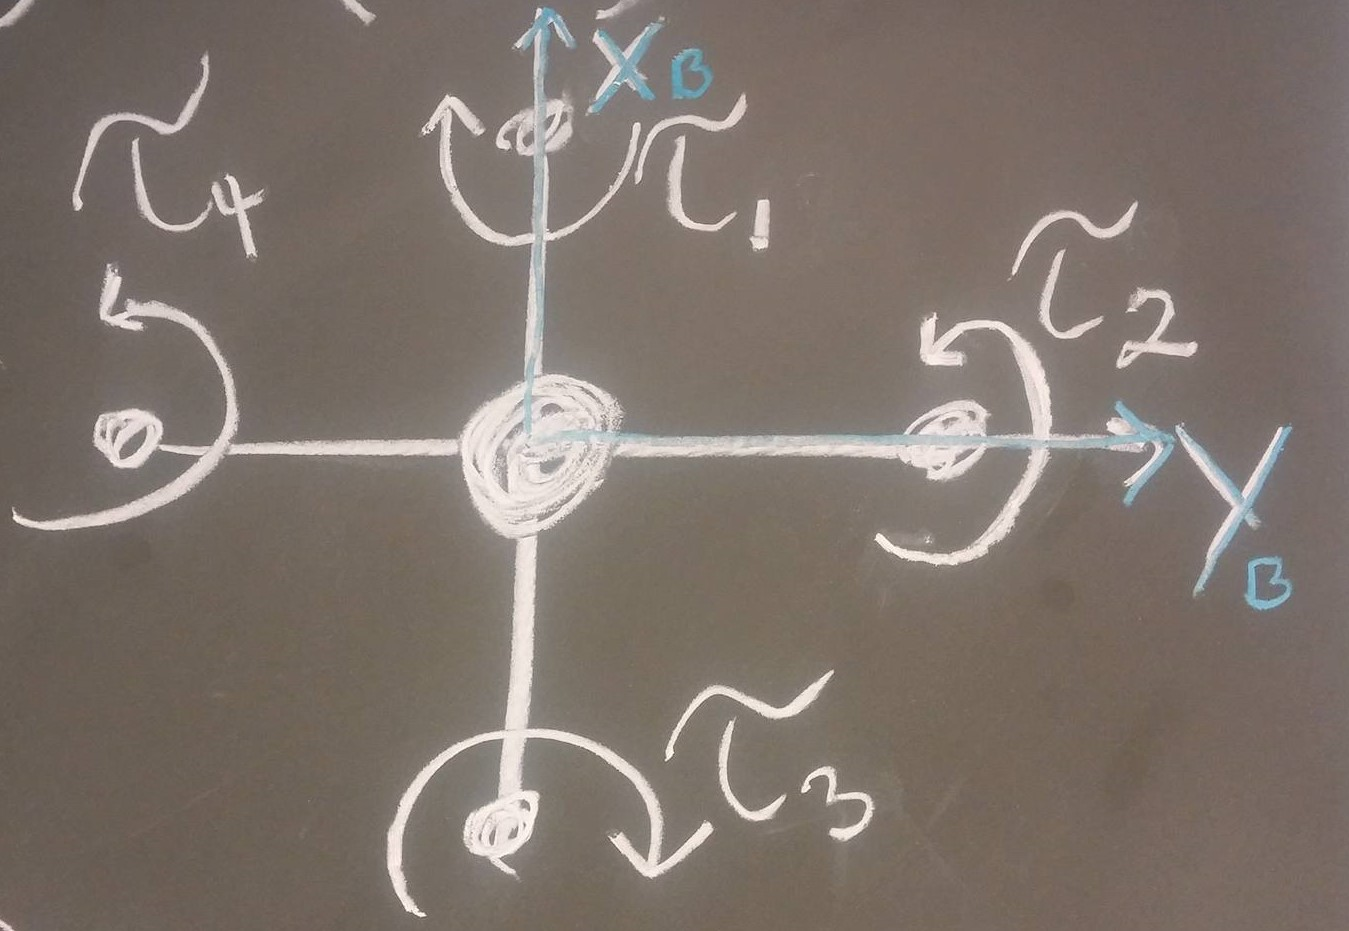
\includegraphics[scale=.15]{figures/torques_diagram}
			\centering
			\captionsetup{justification=centering}
			\captionof{figure}{Diagram of the quadcopter from above, where the references for the drag}}
			\label{PotentiometerResolutionRadDeg}
		\end{figure}
	\end{minipage}
\end{minipage}


\where{
	\va{$\tau_m (t)$}{is the motor torque}{Nm}
	\va{$i_a (t)$}{is the applied current}{A}
	\va{$K_t$}{is the motor constant}{Nm/A}
	\vspace{0.1 cm}
}

